\chapter{Desarrollo}

Para el desarrollo de este Trabajo de Fin de Grado es necesario utilizar múltiples tecnologías y herramientas. En este capítulo se explicará brevemente el estado actual de los chatbots, las distintas herramientas para desarrollarlos, así como los lenguajes de programación utilizados, qué es el procesamiento natural del lenguaje.

Lo primero que hay que tener en cuenta es que se han desarrollado tres servicios desde cero. Por un lado se ha creado una base de datos no relacional, luego una Api Rest para manejar la base de datos y por último un chatbot que será el que consuma la API y a su vez la base de datos. 

\section{Arquitectura del Proyecto}

Este Trabajo de Fin de Grado está incluido dentro de una estructura que está formada por varios proyectos que se explicarán a continuación, así como de las tecnologías seleccionadas para desarrollar el proyecto.
En el ordenador instalado en la estación de Fuenlabrada está colocado el programa \textit{Echoes Watcher} \cite{echoesWatcher}. Este programa lee el archivo de configuración  generado por Echoes para obtener datos de interés (peak, directorio, nombre estación, etc) y según se van generando ficheros de detecciones, el programa mediante un programa de monitorización, lee esos ficheros y en caso de encontrar alguna detección, se envían los datos a través de un Broker MQTT \cite{singh2015secure} al equipo ubicado en el Centro de Supercomputación y Visualización de Madrid (Cesvima).

Todos los días se procede a hacer un backup de los datos sin filtrar a otro computador del proyecto ubicado en la Escuela Técnica Superior de Ingeniería y Diseño Industrial (ESTIDI).

En el Cesvima se encuentra ubicado el programa StreamGenerator \cite{StreamGenerator}. Este programa está suscrito al broker y puede recibir datos de configuración de la estación y datos de las detecciones. Cuando recibe datos de configuración de las detecciones genera un fichero de liquidsoap \cite{liquidsoap} si no existe o si ha cambiado la configuración de la estación. Este fichero liquidsoap genera una lista de reproducción que está ubicada en el Instituto Astrofísico de Canarias y se trata de un bucle infinito de ruido (basado en el archivo de configuración) y a medida que le llegan detecciones de una estación se altera dicha lista de reproducción para añadir los sonidos generados con la detección que recibe del broker, y una vez que el sonido es reproducido, se borra. 
Por cada estación existente hay una lista de reproducción, lo que significa que existe un proceso liquidsoap ejecutándose por cada estación.  

Todos los datos existentes en la estación de Fuenlabrada pasan a través de un Pipeline gestionado mediante \textbf{Apache Airflow}. Este programa es un orquestador de servicios, es decir, es utilizado para automatizar tareas sistemáticas dividiendo estas mismas en subtareas. Los casos de uso más típicos son la automatización de carga de datos, acciones periódicas de mantenimiento y tareas de administración. Para ello permite el uso de herramientas como \textit{cron} y ejecutarlos bajo demanda.
Mediante esta herramienta se envían los datos a un servidor existente en el Departamento de Arquitectura y Tecnología de Sistemas Informáticos. En este servidor existe una base de datos relacional en MySQL donde se almacenan los datos en bruto del programa Echoes. 

Para entender mejor toda la estructura del proyecto, se incluye el siguiente diagrama explicativo.

\section{Arquitectura General del Trabajo}

A continuación, se mostrará la arquitectura en la que se rige este Trabajo de Fin de Grado.

\begin{figure}[h]
    \centering
    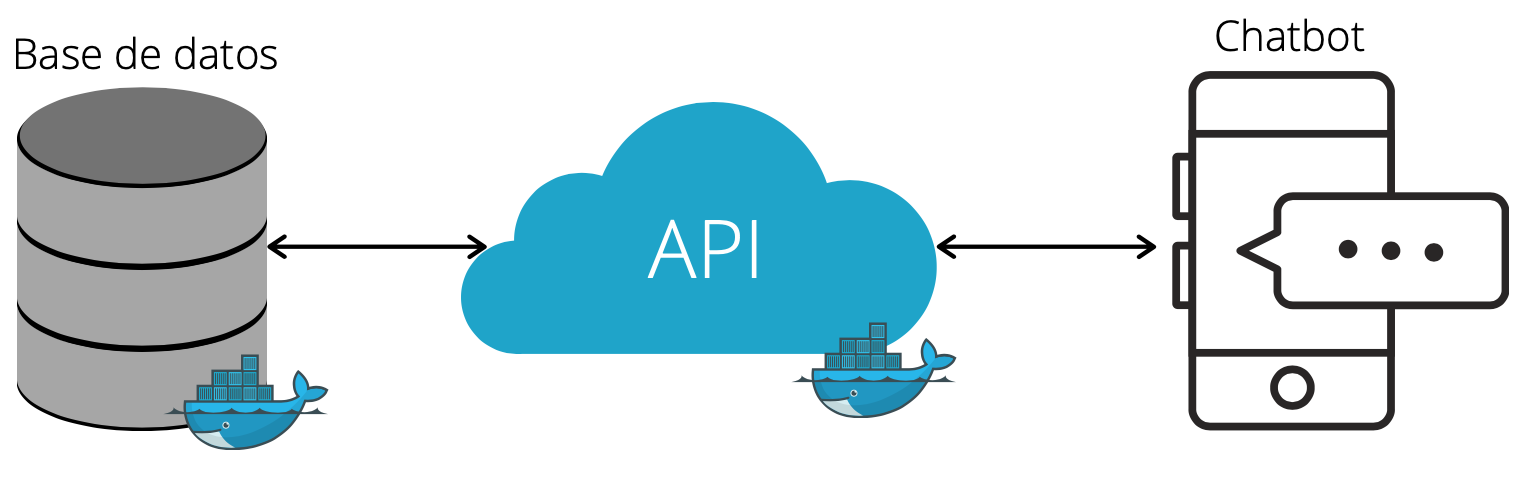
\includegraphics[scale=0.4]{{include/figuras/ArquitecturaGeneral.png}}
    \caption{Arquitectura general}
    \label{fig:arquitectura_general}
\end{figure}

Como se puede observar en la figura \ref{fig:arquitectura_general}, la API RestFul es el software encargado de gestionar e interactuar con la base de datos, sirviendo los datos a los usuarios. Para que el proyecto sea lo más escalable posible se ha decidido separar los servicios de forma que estén débilmente acopladas. 

\subsection{Base de Datos}
Para el proyecto Sonidos del Cielo hemos elegido MongoDB. En gran parte debido a que es una herramienta perfecta para entornos con bajos recursos de computación, no es necesario pagar ningún tipo de licencia, posee una gran comunidad y muy buena documentación, además de muy escalable. La ventaja principal de MongoDB es que los documentos no tienen que seguir una estructura definida, es decir, se puede trabajar con documentos independientes, modificar el contenido de uno de forma individual y no afectar a la estructura.

\begin{figure}[h]
    \centering
    
\includegraphics[scale=0.2]{include/figuras/mongo.png}
    \caption{Logo de MongoDB}
    \label{fig:mongo}
\end{figure}

La característica principal de MongoDB es la velocidad, dado que está escrito en C++ tiene la capacidad de aprovechar los recursos del sistema de una manera eficiente, es decir, tiene un gran balance entre funcionalidad y rendimiento gracias a su sistema de consulta de contenidos. Las características principales de la plataforma son:

\begin{itemize}
    \item Consultas ad-hoc: se pueden realizar todo tipo de consultas. Podemos buscar por campos como si de una base de datos relacional se tratase pero además podemos buscar por rango, mediante expresiones regulares.
    \item Indexación: el concepto es muy parecido al utilizado en las bases de datos relacionales, sin embargo, en MongoDB se puede indexar cualquier campo documentado e incluir múltiples índices secundarios.
    \item Balanceo de carga: MongoDB posee la capacidad de ejecutarse de manera simultánea en múltiples servidores, dando un servicio de balanceo de carga o de replicación de datos, de manera que es posible mantener el funcionamiento del sistema en caso de un fallo de hardware.
    \item Almacenamiento de archivos: puede ser utilizado también como almacenamiento de archivos, esta función, conocida como GridFS está incluida en la distribución oficial y permite manipular archivos y su contenido.
    \item Ejecución de JavaScript en el lado del servidor: es posible realizar consultas utilizando código escrito en JavaScript, haciendo que estas sean enviadas directamente a la base de datos para ser ejecutadas.
\end{itemize}

\subsubsection{Funcionamiento de MongoDB}
MongoDB está orientado a documentos. Esto significa que en lugar de guardar los datos en registros se guardan en documentos BSON, que no es otra cosa que un fichero JSON binario.
Esto es una de las grandes diferencias respecto a las bases de datos relacionales. 
MongoDb se compone de colecciones que a su vez está formado por documentos documentos. 

Si hiciésemos una comparación con los elementos de una base de datos relacional, se trataría de una tabla. Dentro de cada colección existen múltiples documentos que están compuestos de pares Clave-Valor. 
La principal diferencia respecto a una base de datos relacional es que no es necesario que los documentos de una misma colección tengan el mismo formato ni los mismos campos.

\subsubsection{Arquitectura de la Base de Datos}

Las tablas obtenemos desde ficheros que se encuentran en un servidor del Spanish Virual Observatory (SVO) dentro del Departamento de Arquitectura y Tecnología de Sistemas Informáticos de la Escuela Técnica Superior de Ingenieros Informáticos de la Universidad Politécnica de Madrid. A partir de este fichero se crean las tablas que se aprecian en la figura \ref{fig:tablas_base_datos}

\begin{figure}[H]
    \centering
    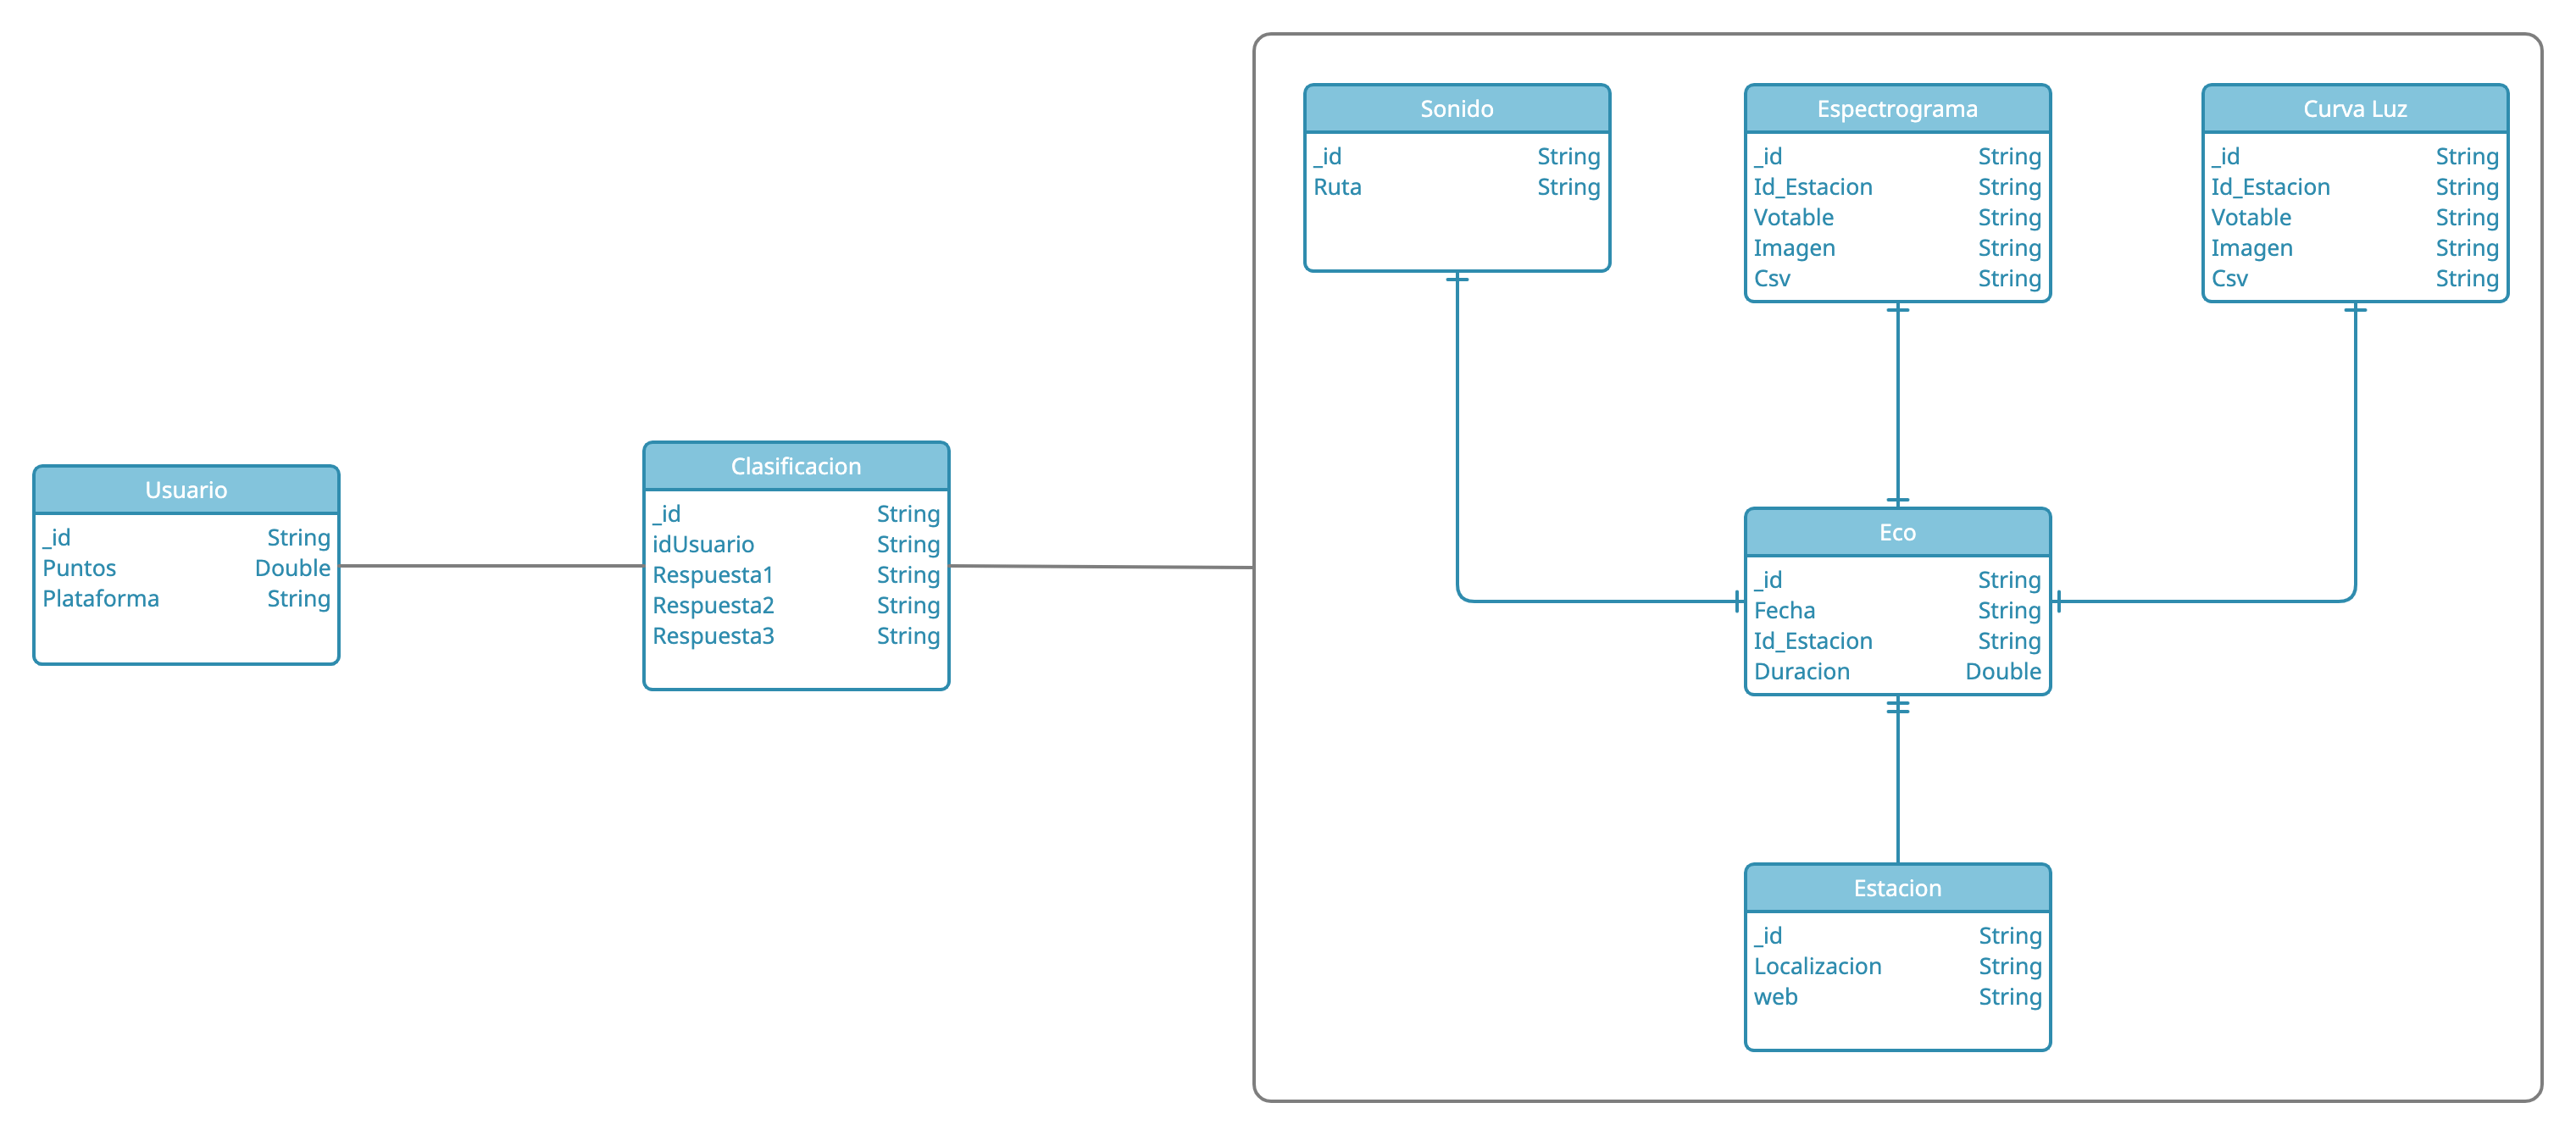
\includegraphics[width=\textwidth]{include/figuras/Tablas.png}
    \caption{Colecciones de la base de datos}
    \label{fig:tablas_base_datos}
\end{figure}

Aunque hemos explicado anteriormente que no es estrictamente necesario que existan relaciones entre las tablas, en este proyecto si que es necesario puesto que varias tablas proceden del mismo meteoroide.

Una vez creada la base de datos y establecer usuarios para restringir el acceso a la misma, podemos realizar operaciones de consulta, inserción, eliminación y actualización de documentos, colecciones y bases de datos a través de la consola incluida dentro del paquete de instalación de MongoDB. 

\begin{figure}[H]
    \centering
    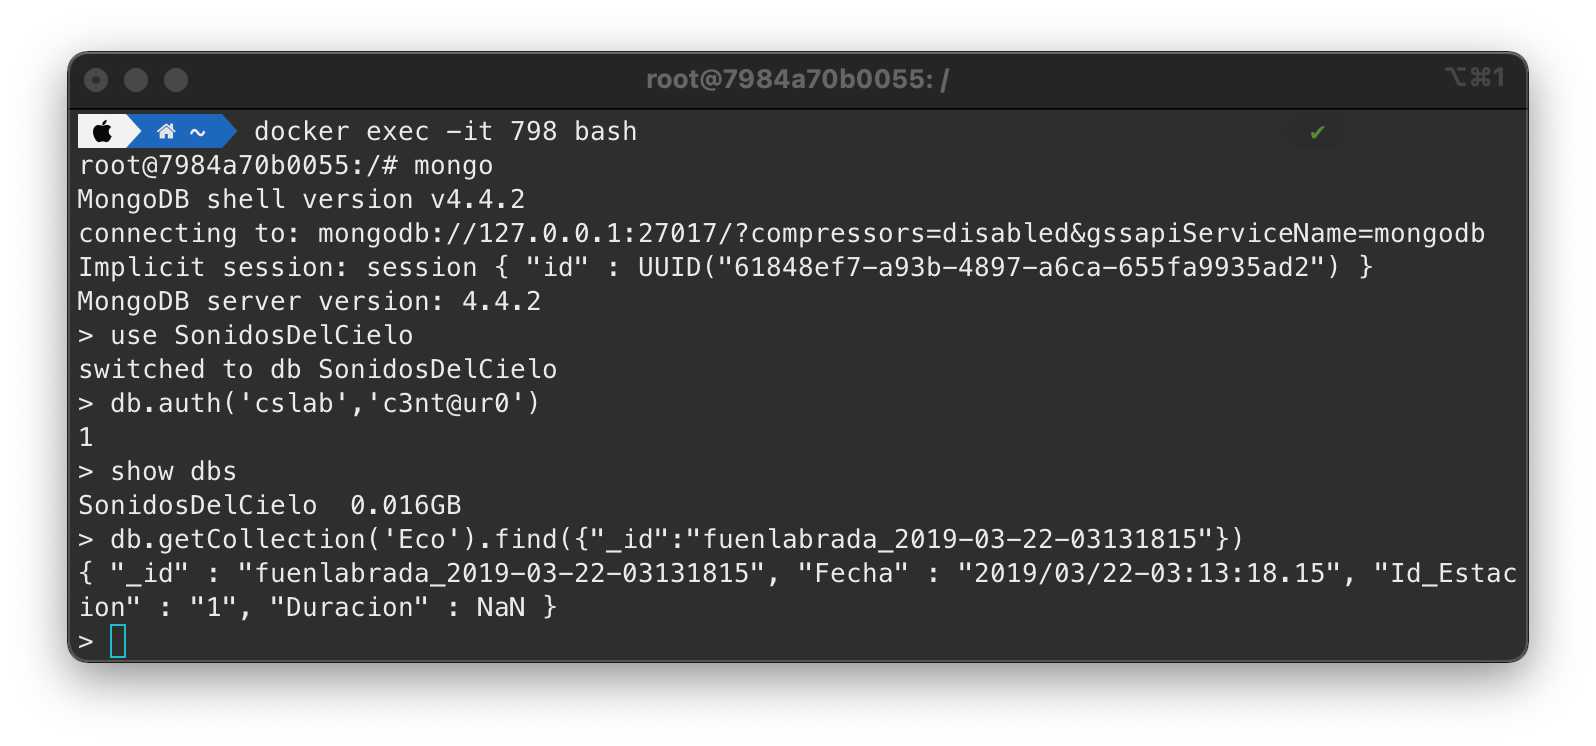
\includegraphics[scale=0.4]{include/capturas/TerminalMongo.png}
    \caption{Operación con terminal de mongo}
    \label{fig:terminal_mongo}
\end{figure}

También existen herramientas gráficas para modificar cualquier parámetro de una base de datos en Mongo como puede ser MongoDB Compass o Robo 3T. Estas herramientas proporcionan una vía más sencilla y visual para trabajar con las bases de datos además de no tener que aprender o buscar dentro de la documentación los comandos necesarios para manejar una interfaz de línea de comandos propietaria. Aunque también nos permite el ejecutar comandos como si se tratase del terminal como se puede observar en la figura \ref{fig:robo3t}.

\begin{figure}[H]
    \centering
    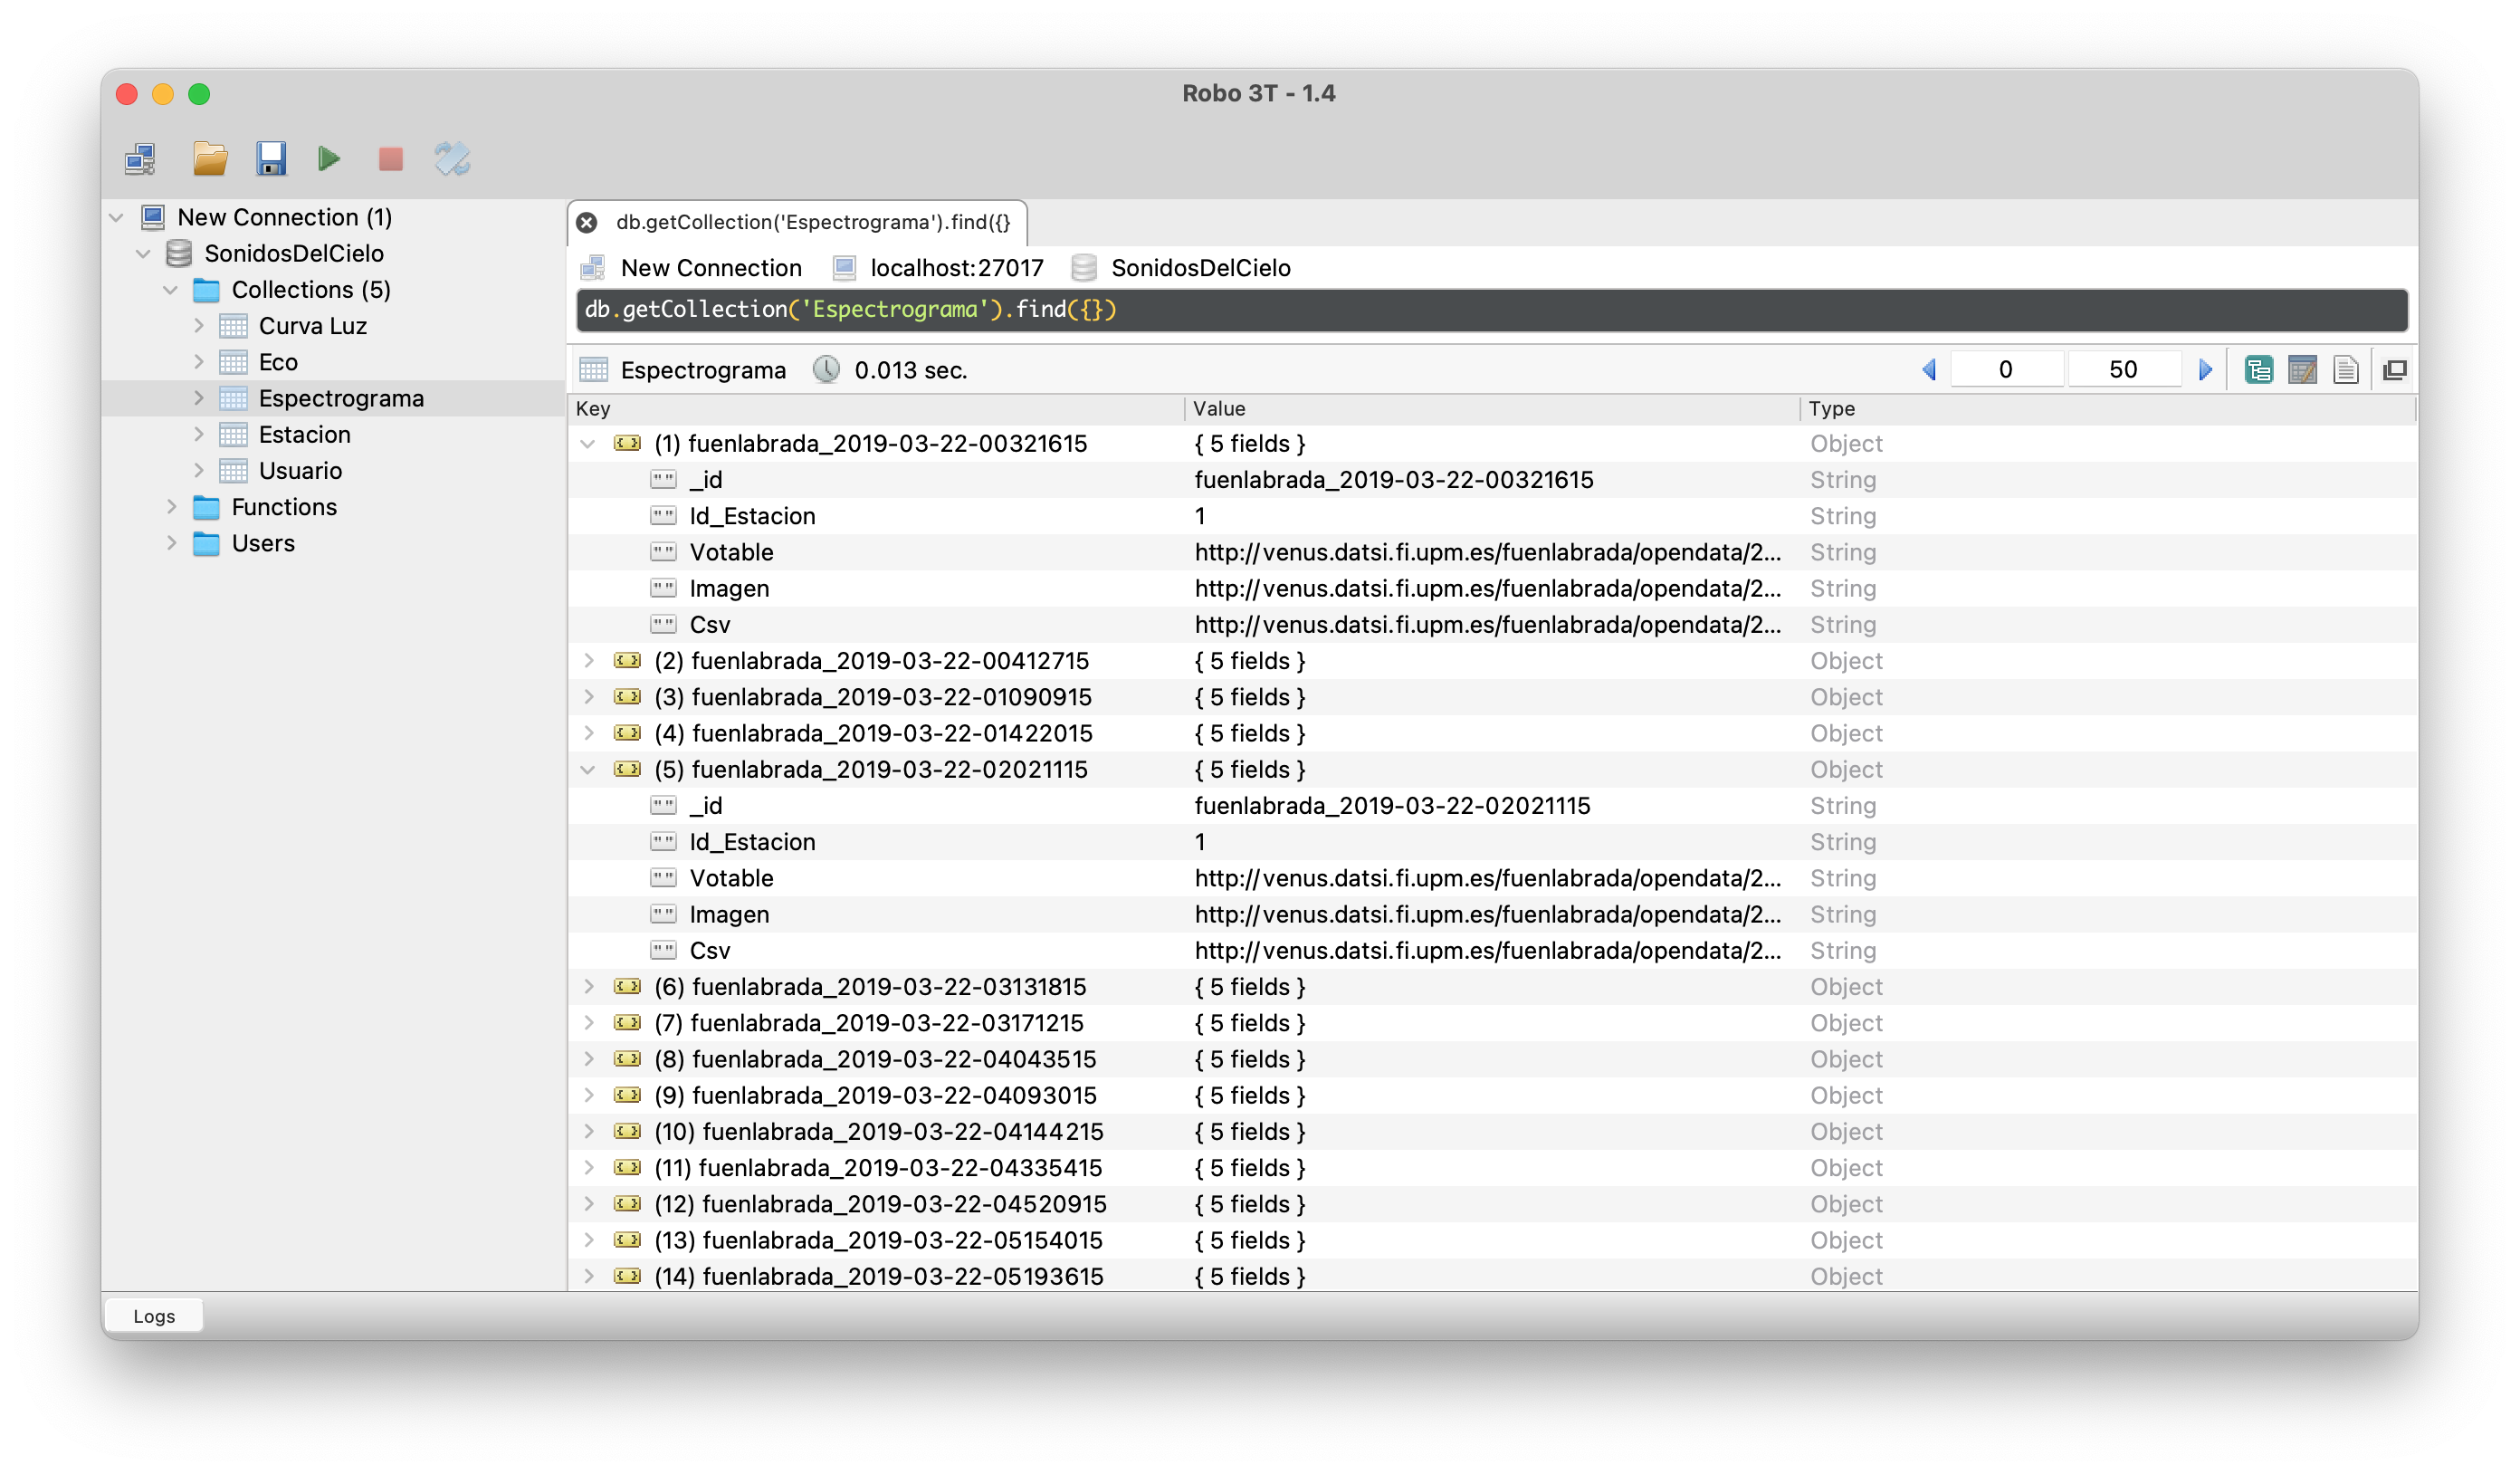
\includegraphics[scale=0.3]{include/capturas/Robo3T.png}
    \caption{Interfaz de Robo3T}
    \label{fig:robo3t}
\end{figure}

\newpage
\subsection{Lenguaje de Programación Python}

Tanto para la carga de los documentos en la base de datos como para el desarrollo del chatbot ha sido necesario el uso del lenguaje de programación Python. Python es un lenguaje de programación creado a finales de los años 80 por Guido van Rossum en el Centro para las Matemáticas y la Informática de Países Bajos. Este lenguaje posee una gran flexibilidad que produce código ordenado, limpio y fácilmente legible. Sus principales características pueden resumirse en las siguientes\cite{python}:

\begin{figure}[h]
    \centering
    
\includegraphics[scale=0.4]{include/figuras/python.png}
    \caption{Logo de Python}
    \label{fig:Python}
\end{figure}

\begin{itemize}
    \item Gratis: No es necesario pagar licencia para utilizarlo
    \item Interpretado: se ejecuta sin tener que pasar por un compilador y los errores son detectados en tiempo de ejecución.
    \item Multiplataforma: está disponible para Windows, Mac y Linux. 
    \item Tipado dinámico: las variables declaradas se comprueban durante el tiempo de ejecución.
    \item Multiparadigma: soporta programación funcional, programación imperativa, declarativo, modular, dirigido a eventos, programación asíncrona, lógico, estructurado, con restricciones y programación orientada a objetos.
\end{itemize}

Es un lenguaje que se tiene una curva de aprendizaje muy rápida, además cuenta con una gran comunidad lo que hace que existan librerías y módulos especializados desarrollados como \textit{pandas} (tratamiento de datos) \textit{librosa} (para procesamiento de audio), \textit{sklearn} (machine-learning) o frameworks como \textit{Django} (para desarrollo web) o en nuestro caso, \textbf{RASA} para desarrollar un chatbot. 

\subsection{Arquitectura aplicación RestFul}

La aplicación RestFul no es más que el software que hace de intermediario para enviar información de la base de datos al cliente o para insertar datos desde el cliente a la base de datos. El cliente es aquel que consume la información, en nuestro caso, el chatbot. El servidor se ha desarrollado en Node.js. Fue diseñado para la construcción de aplicaciones escalables, siendo un punto muy a favor para nuestra elección. 

\begin{figure}[h]
    \centering
    
\includegraphics[scale=0.15]{include/figuras/node.jpg}
    \caption{Logo de Node.js}
    \label{fig:node}
\end{figure}

\subsubsection{Funcionamiento de Node.js}

Node.js es un entorno de ejecución de JavaScript \cite{javascript} orientado a eventos asíncronos. Comparándolo con servicios web clásicos donde cada nueva conexión genera un nuevo subproceso (ocupando memoria RAM del sistema) y normalmente ocupando toda la memoria RAM disponible. Node.js trabaja en un subproceso únicamente, utilizando el modelo entrada y entrada sin bloqueo de la salida, esto permite soportar una cantidad enorme de conexiones simultáneas mantenidas dentro del bucle de eventos. El servidor consta de un subproceso que trata un evento tras otro.
Cuando se produce una nueva solicitud se genera un evento. El servidor comienza a procesarlo y cuando se produce una operación de bloqueo de la entrada/salida, no espera a que se termine sino que se crea una \textit{función de callback}. El servidor comienza instantáneamente a procesar otro evento y cuando termine la operación de entrada/salida, seguirá trabajando en la solicitud ejecutando la función de callback tan pronto como sea posible.

Gracias a este mecanismo, el servidor no necesita crear subprocesos lo que significa que no tiene apenas sobrecarga. Además, puesto que queremos tratar las peticiones de los usuarios, la mejor manera de hacerlo es de forma asíncrona así no es necesario esperar a que se traten las peticiones realizadas con anterioridad.


\subsubsection{Ventajas de utilizar Node.js}

Node.js es la plataforma de software más utilizada en la actualidad por encima de otros entornos de ejecución y lenguajes de programación como pueden ser C o PHP a la vez que tiene un tiempo de ejecución mucho mayor. No es un lenguaje de programación complejo pero requiere una mayor comprensión y cantidad de líneas de código que PHP. Cuando hablamos de Node.js hay algo que es necesario destacar, el conocido como Node Package Manager (NPM) que viene por defecto con la instalación de Node.js.


\subsubsection{Librerías utilizadas}A continuación se especificarán los paquetes utilizados para el desarrollo de la API RestFul.

\begin{itemize}
    \item Async: es un módulo que proporciona funciones sencillas para el tratamiento de llamadas asíncronas.
    \item Body-parser: es un middleware encargado de extraer todo el cuerpo de una request entrante y la muestra en el \textit{req.body} 
    \item Cors: este paquete se encarga de controlar el mecanismo que utilizan las cabeceras HTTP para permitir que un \textit{user agent} tenga permiso para acceder a ciertos recursos desde un servidor en un dominio distinto al que pertenece.
    \item Dotenv: Sirve para cargar variables de entorno desde un fichero .env.
    \item Express: es un framework de desarrollo web inspirado en Sinatra y por consiguiente, el estandar de la gran mayoría de aplicaciones de Node.js. Es la librería que utilizaremos para desplegar el servidor de la API.  
    \item Mongoose: es una herramienta encargada del tratamiento de bases de datos MongoDB de manera asíncrona.
    \item Nodemon: este paquete simplifica la tarea de volver a iniciar la aplicación cada vez que se realice un cambio en el código. Es un demonio que se ejecuta en segundo plano y es el encargado de comprobar los cambios e iniciar el servidor.
    \item Swagger-Jsdoc: genera definiciones OpenAPI a partir de comentarios JSDoc.
    \item Swagger-UI-Express: crea la interfaz de usuario de Swagger en base a las definiciones creadas con Swagger-JSDoc.
\end{itemize}

\subsection{Visual Studio Code}

Visual Studio Code es un editor gratuito y de código abierto desarrollado por Microsoft y que se distribuye mediante licencia MIT. \footnote{Licencia MIT: licencia creada en el Instituto Tecnológico de Massachusetts, se trata de una licencia de software libre que impone muy pocas restricciones en su reutilización} Se trata de un software multiplataforma (Windows, macOS y Linux).
Está creado en NodeJS y Electron \cite{electron} y con Blink como motor gráfico.

Se trata de un editor hackeable, es decir, permite modificar el comportamiento del editor completamente (tema del editor, atajos de teclado, preferencias, etc), tiene soporte para Git integrado, autocompletado de código, terminal integrado y debugger.

Además posee una biblioteca de extensiones \ref{fig:vscode} mediante la cual puedes añadir herramientas que ayuden en los proyectos o visualizar el código de forma más eficiente. También posees un live server a través del cual puedes visualizar código web en tu navegador predeterminado inmediatamente según guardas el código sin ser necesario refrescar.

\begin{figure}[h]
    \centering
    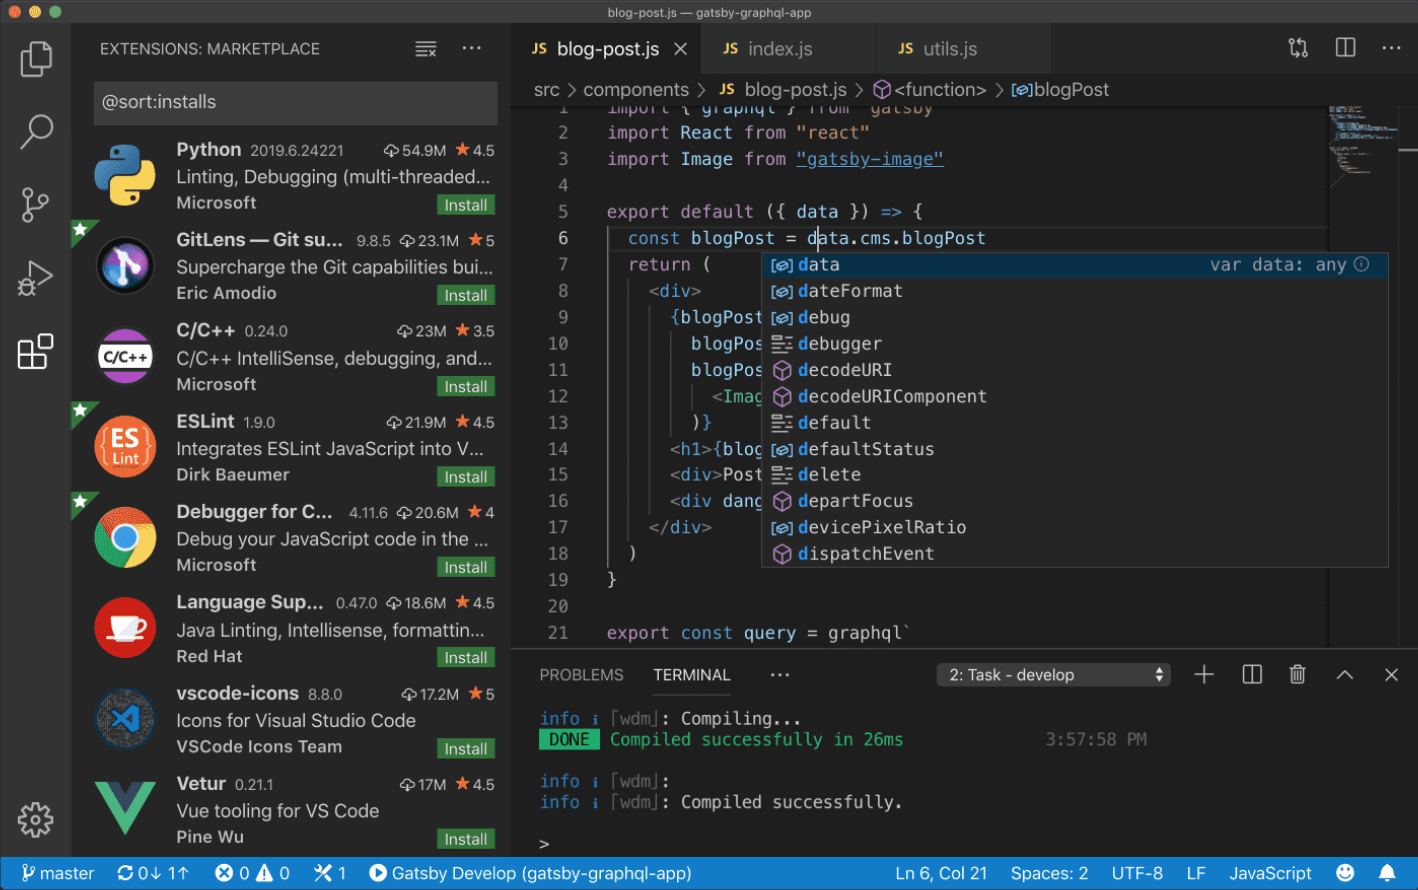
\includegraphics[width=\textwidth]{include/figuras/VSCode.png}
    \caption{Visual Studio Code}
    \label{fig:vscode}
\end{figure}

A continuación se explicará brevemente las extensiones utilizadas:.

\begin{itemize}
    \item \textbf{Docker}: esta extensión simplifica la forma en la que construir, controlar y desplegar aplicaciones \textit{dockerizadas}, además proporciona herramientas dentro de un contenedor para realizar debugging de aplicaciones desarrolladas en Node.js, Python y .NET Core.
    \item \textbf{YAML}: proporciona compatibilidad completa con el lenguaje YAML con compatibilidad para la sintaxis de Kubernetes.
    \item \textbf{MarkdownLint}: incluye una biblioteca de reglas para entender los estándares y la coherencia de los archivos Markdown. 
    \item \textbf{TODO Tree}: esta extensión busca rápidamente las etiquetas TODO y FIXME y las muestra en un árbol. 
\end{itemize}


\subsection{Git y Github}


En el desarrollo de cualquier proyecto de software surge la necesidad de gestionar los cambios que se producen entre versiones diferentes de un mismo código fuente. Habitualmente este proceso se inicia utilizando sufijos en los ficheros que se modifican (v1, antiguo, nuevo) pero este proceso no es ni eficiente ni práctico, mucho menos si trabajamos en equipo, dando lugar a la eliminación de archivos válidos realizados por otros componentes del equipo, incapacidad de conocer que cambios se han realizado, etc.

En todo proyecto, más tarde o más temprano aparece la necesidad de trabajar en distintas ramas, en el entorno empresarial suelen ser desarrollo y producción. En la rama de desarrollo se procede a introducir las nuevas modificaciones y en la rama de desarrollo las versiones estables del programa.

Para ayudarnos con esta tarea aparecen soluciones como Git, CVS que realizan tareas fundamentales como pueden ser:

\begin{figure}[h]
    \centering
    
\includegraphics[scale=0.1]{include/figuras/Git.png}
    \caption{Logo de Git}
    \label{fig:git}
\end{figure}

\begin{itemize}
    \item Comparación de ficheros de tal manera que rápidamente encontremos las diferencias entre los dos. 
    \item Restauración de versiones anteriores.
    \item Fusionar versiones.
    \item Trabajar con varias ramas de un proyecto.
    \item Facilitar la colaboración.
\end{itemize}


En el caso del proyecto Sonidos del Cielo la herramienta de control de versiones utilizada ha sido \textbf{Git}. 

Git surgió de la mano de Linus Torvals \cite{torvalds2005git}, es un sistema de control de versiones de código abierto, multiplataforma, lo que nos permite crear repositorios en cualquier sistema operativo. Existen gran variedad de herramientas gráficas para manejar Git pero lo más utilizado el la línea de comandos dado que, una vez aprendidos los comandos básicos, nos permite realizar las operaciones con mayor velocidad. 

Github es un servicio para alojar repositorios creado en San Francisco en el año 2008. Está pensado para compartir código fuente en cualquier lenguaje de programación y dejarlo a disposición de cualquiera que quiera reutilizarlo siempre y cuando haya permiso para ello. Si cualquier otro usuario que no sea el creador del proyecto puede realizar un \textit{fork}, un fork no es otra cosa sino que la creación de una copia de otro proyecto en otro repositorio.
También hay repositorios privados en los que sólo el creador del repositorio y las personas a las que el de acceso podrán participar.

\begin{figure}[h]
    \centering
    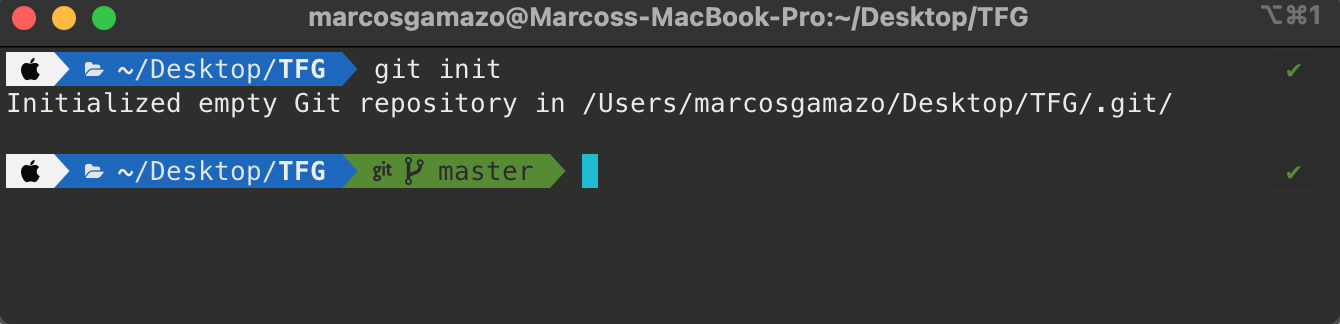
\includegraphics[width=\textwidth]{include/capturas/gitInit.png}
    \caption{Inicialización de repositorio en Git}
    \label{fig:git_init}
\end{figure}


Github cuenta con diversas herramientas de las que las más destacables son:

\begin{itemize}
    \item Gollum: permite la creación de wikis basadas en git.
    \item Sistema de revisión de código: para añadir comentarios y discutir sobre las modificaciones realizadas.
    \item Visor de ramas: dónde podremos revisar los avances del repositorio.
    \item Herramienta de seguimiento de problemas: nos permite abrir tickets de incidencias o mejoras a realizar.
\end{itemize}


\subsection{Swagger}
Una de las partes más importantes en cualquier proyecto es la documentación del código. Es muy habitual en nuestro campo que hay que modificar, mantener o simplemente que utilizar código desarrollado por otra persona y se convierte en una tarea ardua que obliga a invertir demasiado tiempo en comprenderlo. 

Para evitar estas situaciones es habitual adaptar herramientas que permitan comentar el código fuente del software que desarrollemos de tal manera que sea legible por cualquier persona. En el proyecto Sonidos del Cielo se ha decidido seleccionar la herramienta \textit{Swagger} para documentar la API RestFul. 

Swagger se compone de una serie de herramientas, reglas y especificaciones mediante las cuales podremos documentar y probar una API de una manera sencilla. La principal baza para utilizar Swagger es que es realmente sencilla de implementar y cualquier persona es capaz de entenderlo, tenga conocimientos de programación o no. Esto es posible gracias a \textbf{Swagger UI}, es una de las características más importantes de la plataforma, esta herramienta nos permite organizar las operaciones CRUD de la API basándose en los ficheros YAML o JSON y creando un entorno interactivo.

\begin{figure}[H]
    \centering
    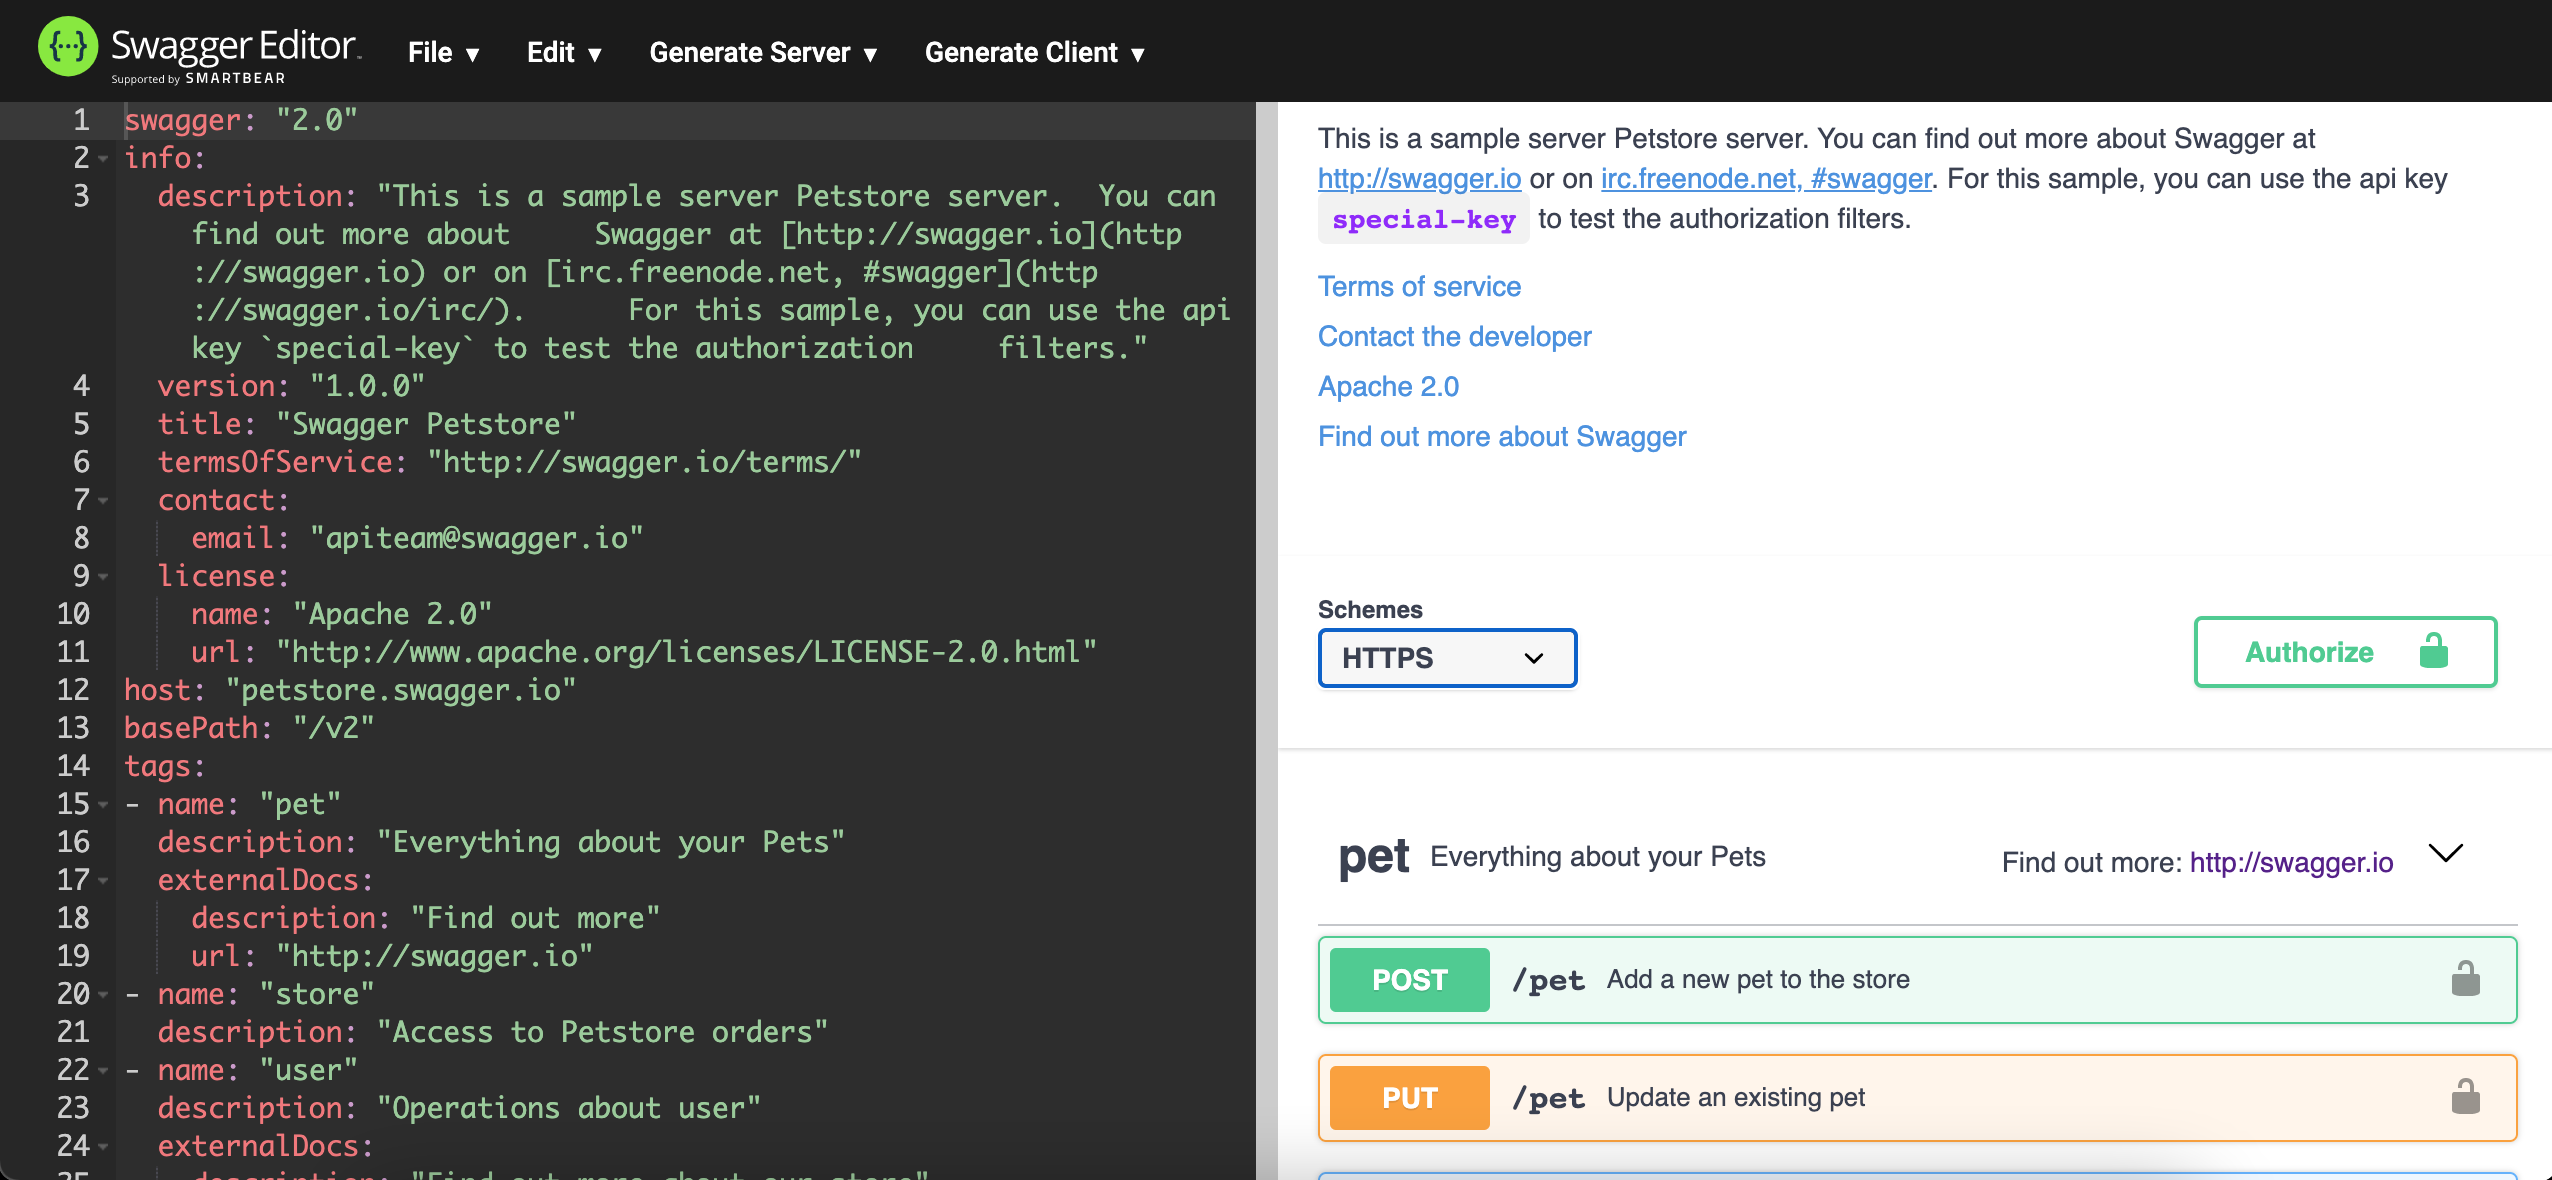
\includegraphics[width=\textwidth]{include/capturas/SwaggerEditorOnline.png}
    \caption{Swagger Editor}
    \label{fig:swagger_online}
\end{figure}

Para esta tarea podemos utilizar la versión del editor en línea, \textit{Swagger editor} que proporciona la plataforma como se muestra en la figura \ref{fig:swagger_online}, esta herramienta nos indicará los errores que se hayan cometido y además brindará sugerencias y alternativas para mejorar la documentación.

Nuestra implementación pasa por la utilización de Swagger y Swagger UI como varios paquetes instalables dentro de Node.js a través del instalador npm. Dentro de la definición del servidor se incluyen las opciones del servidor como se muestra en la figura \ref{fig:swagger_options} entre las que cabe destacar la versión del API Rest, la versión OpenAPI o la información del proyecto.

\begin{figure}[H]
    \centering
    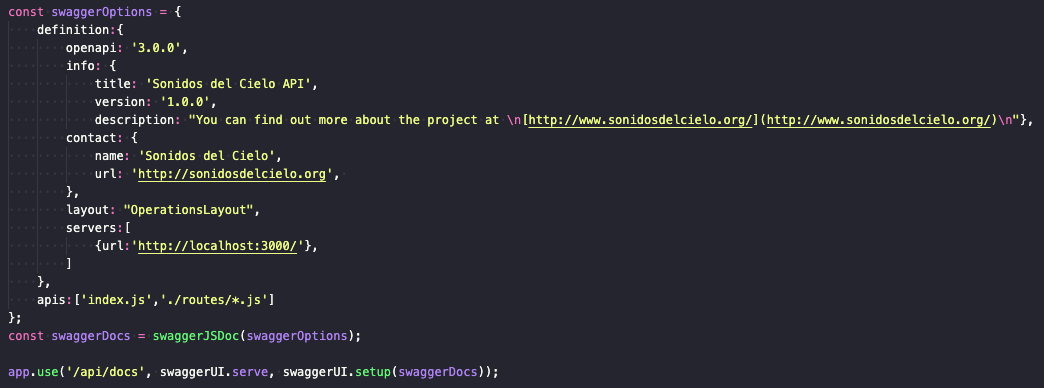
\includegraphics[width=\textwidth]{include/capturas/SwaggerOptions.png}
    \caption{Opciones del servidor de Swagger}
    \label{fig:swagger_options}
\end{figure}

Una vez establecido los parámetros básicos del servidor y haber definido los componentes que forman la API Rest es momento de añadir el código YAML para crear la documentación de los distintos métodos. En ese código se indica el tipo de formato que se produce, \textbf{JSON} en nuestro caso, los códigos de respuesta que proporciona la API.

\begin{figure}[h]
    \centering
    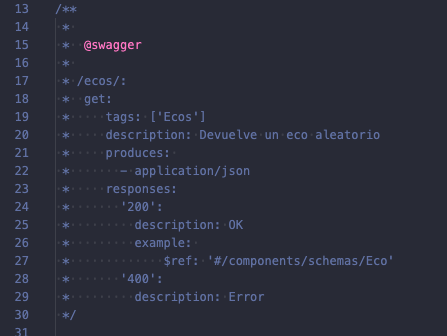
\includegraphics[scale=0.7]{include/capturas/SwaggerYAML.png}
    \caption{Definición Swagger}
    \label{fig:swagger_definition}
\end{figure}

Una vez estén comentados todos los métodos de nuestra API, se genera una interfaz gráfica similar a la mostrada en la figura \ref{fig:swagger_online} en el \textit{endpoint} que hayamos definido en dónde se pueden probar los métodos comentados a lo largo del código.

\subsection{Postman}
